\documentclass[11pt]{article}
\usepackage{amsmath}
\usepackage{graphicx}
\usepackage{float}
\usepackage{blindtext}
\usepackage{subcaption}
\usepackage[a4paper,width=180mm,top=22mm,bottom=22mm]{geometry}
\usepackage{fancyhdr}
\usepackage{longtable}
\usepackage[
    backend=biber,
    style=ieee
]{biblatex}
\usepackage{xcolor}
\usepackage{soul}
\usepackage{listings}

\newcommand{\hlc}[2][yellow]{{%
    \colorlet{foo}{#1}%
    \sethlcolor{foo}\hl{#2}}%
}


\addbibresource{report.bib}

\graphicspath{ {./images/} }

\pagestyle{fancy}
\fancyhead[C]{EEE3027}
\fancyhead[L]{EEE3027 Final Essay}
\fancyhead[R]{16th of May}

\cfoot{} % get rid of the page number 
\fancyfoot[L]{6596386}
\fancyhead[C]{}
\fancyfoot[R]{\thepage}

\begin{document}
\begin{titlepage}
    \begin{center}
    
\includegraphics[width=\textwidth]{Logo.png} % also works with logo.pdf
    \vfill
    \Huge
    \textbf{EEE3027: Final Essay}
    \vfill
    \huge
    \vspace{1cm}
    \Large
    16th of May 2023\\
    URN: 6596386\\
    \vfill
    \vfill
    \Large
    School of Computer Science and Electronic Engineering\\
    Faculty of Engineering and Physical Sciences\\
    University of Surrey\\
    \end{center}
\end{titlepage}

\renewcommand{\thesection}{\Alph{section}}
\renewcommand{\thesubsection}{\Alph{section})\alph{subsection}}

\pagenumbering{Roman}
%\begin{abstract}

\vspace{1cm}
%\end{abstract}
\tableofcontents
\pagebreak

\pagenumbering{arabic}
\section{System on a Chip Interfacing}
\subsection{JTAG Advantages}
As chips have become denser, directly probing pins, such as with the old bed-of-nails technique, is no longer possible, yet accessing these pins is vital for testing.
This is the problem the Joint Test Action Group set out to solve with JTAG, which is a specification for accessing on-ship resources and boundary-scan hardware testing on the board\cite{jtag_tutorial}.
Without boundary-scanning, the only test option is functional, which requires massive amounts of test cases to exhaust all possibilities and does not help find the cause of a failure.
Meanwhile, JTAG's boundary scan enables one to control and monitor individual IO pins, allowing for structural tests. 
Structural tests will help find assembly defects, such as shorts, and run much quicker as they are non-exhaustive.

JTAG also offers other benefits, such as monitoring systems during operation without disrupting them and even testing systems that are otherwise non-functional\cite{Corelis}.
This is because JTAG is independent of the system and accessible via just four pins (depending on specification).
As the logic and pins are part of the IC, JTAG will allow for testing throughout a product's life cycle.
Engineers can use the interface during prototyping, production, and after deployment\cite{Corelis}.
JTAG also daisy chains, allowing multiple devices within a system to be tested with one interface.

(208)


\subsection{JTAG Functionality}
The JTAG implementation shown in Figure 1 of the essay brief connects to the internal bus of the ARM Cortex-M0 SoC.
This connection enables the JTAG interface to control and monitor the data on that bus, allowing one to shift in a test pattern to test
the NVIC, processor core, debug subsystem, memory and peripherals, or any combination thereof. 

This sort of boundary testing is done via a path of interconnected shift-register cells on each signal pin in the bus, which are controlled via the Test Access Port (TAP) of the JTAG.
The TAP has four core control signals\cite{jtag}:
\begin{itemize}
    \item TCK, clock to synchronize operation
    \item TMS, mode select line
    \item TDI, input shifted into cells on the rising edge
    \item TDO, output shifted out of cells on the falling edge 
    \item (Optional) TRST, a reset for the state machine 
\end{itemize}

Creating this functionality in VHDL is done by creating a state machine, shown in Figure \ref{fig:sm}, which is controlled by the value of TMS during the rising edge of TCK.
The state machine has two paths to capture and control the data on the instruction registers (IR) or the data registers (DR).

\begin{figure}[H]        
    \centering
    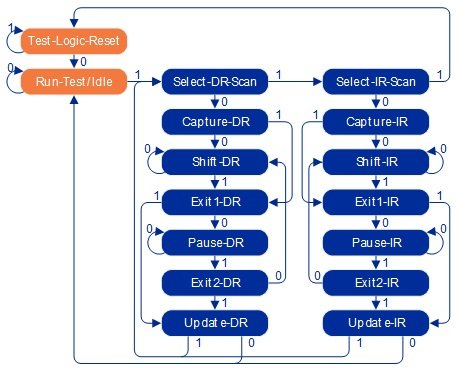
\includegraphics[width=.5\textwidth]{JTAG-state-machine-diagram1.jpg}
    \caption{JTAG State Machine Diagram from Corelis\cite{Corelis}}
    \label{fig:sm}
\end{figure} 

The cells must also be created in VHDL using multiplexers and latches. 
These cells have a parallel input and output, which allow for the regular operation of the device, and shift inputs and outputs, which are used during tests to load data in or read data out.

(235)


\subsection{VHDL Implementation}
Various VHDL implementation concepts can be used to create a low-latency JTAG implementation.
As a whole JTAG throughput can be increased via parallelizing and pipeline, which involved doing multiple operations in parallel and breaking one operation into stages respectively.
Parallelizing is well suited to combinational logic while pipelining lends itself to sequential logic.
However, neither of these method decrease latency instead just increases system throughput.
The main areas to optimize for latency in JTAG are the shift registers and the finite state machine driving the JTAG logic.

As mentioned the TAP in JTAG functions with a state machine, which can be optimized in different ways.
The finite state machine can be split into next-state logic, state memory, output logic, and output register.
Next-state logic has a sensitivity list of only the TMS line, and on the rising edge of the clock, its output will be saved as the current state in the state memory.
Splitting it like this allows reduces the fan-out and the amount of resources that need to be used.
The state can also be stored as a 4-bit integer (as there are 16 states), assuming this system does not need to use one-hot encoding as it is for testing.
Finally for the state machine implementing asynchronous reset, meaning that the rest will occur regardless of the clock, will help as it allows quicker resetting between tests.

A lot of the latency in JTAG occurs while data is being shifted into or out of the shift registers (both the instruction and the data registers.)
To speed this up a specific type of shift register, the barrel shifter, can be used.
Barrel shifters are purely combinational, consisting essentially of sequences of multiplexers, and can shift a specific number of bits over which can be useful for quickly loading and unloading.
This would also require some logic on the TDI line as data comes in only 



\subsection{Calculations Single Stage} \label{sec:single}
% In 300 words or less, calculate the throughput, latency, and clock period of a single-
% stage generic processor that takes 24 ns per instruction. Assume flip-flops at the input
% and out have a treg time of 300 ps.

One can calculate throughput, latency, and clock period given time per unit of work and the register overhead.
Throughput ($\Theta$) is the number of tasks a module can solve in a given period of time, with a standard unit of mega-operations (millions of operations) per second or mops\cite{dally}.
Latency ($T$) is the time taken per task\cite{dally}. 
These two values are reciprocal ($\Theta = \frac{1}{T}$).
The clock period ($T_{\text{clk}}$) is the time from one rising edge to the next

For a generic single-stage processor, which takes 24 ns per instruction ($T_m$), and with flip-flops at the input and output, with 300 ps overhead($t_{\text{reg}}$), the following values can be calculated:

\begin{align}
    T &= T_m + t_{\text{reg}} = 24\text{ ns} + .3\text{ ns} = 24.3\text{ ns}\\
    \Theta &= \frac{1}{T} = \frac{1}{24.3} = 41.15\text{ Mops}\\
    T_{\text{clk}} &= 24.3\text{ ns}
\end{align}

This system area usage could also be calculated if the area of the module ($a_m$) and the area of the register ($a_{\text{ref}}$) were known, using the following equation.
\begin{align}
    a &= a_m + a_{\text{ref}}
\end{align}
(133)

\subsection{Calculations Four Core}
% In 300 words or less, repeat the calculations in (d) and evaluate for an 4-core multi
% ARM processor system and with a 9-stage pipeline. Comment with comparisons from
% (d) on the advantages of using a multi-core pipeline system design and the impact on
% area.

This part expands on part \ref{sec:single} with a four-core system with nine stages.
To create such a system the original module must both be pipelined and parallelized.
Pipelining involves taking a large operation and breaking it into submodules,
this means that submodules will not be idle long as they can begin processing new data as soon as they finish the previous task.
This helps increase throughput at the cost of needing registers between the submodules.
Parallelizing simply duplicates the entire module to allow multiple operations to be done at the same time.
This will increase throughput by a factor of how many parallel systems exist.
However, this comes at the cost of needing to replicate the entire module

For the given example, to find the new throughput, latency, and clock period,
the effect of using nine stages ($n = 9$) must first be calculated.
This has to account for the added register overhead\cite{dally} ($T_m$ and $t_{\text{reg}}$ are unchanged).
\begin{align}
    T &= T_m + nt_{\text{reg}} = 24\text{ ns} + 9*.3\text{ ns} = 26.7\text{ ns}\\
    \Theta_{\text{pipeline}} &= \frac{1}{T_m/n+t_{\text{reg}}} = \frac{1}{24\text{ ns}/9+.3\text{ ns}} = \frac{1}{2.967\text{ ns}} = 337.08\text{ Mops}\\
    T_{\text{clk}} &=  26.7\text{ ns} / 9 = 2.967\text{ ns}
\end{align}

This nine-stage pipelined process can now be parallelized.
The four-core nature of the new system does not add any timing overhead but will increase throughput four-fold, as the task will be completed in parallel.
\begin{align}
    \Theta = \Theta_{\text{pipeline}} * 4 = 337.08\text{ Mops} * 4 = 1348.31 \text{ Mops}
\end{align}

These changes make the new system 32 times faster than the one in part \ref{sec:single}.
The cost of this new design's performance is a considerable increase in area.
The new requirement can be calculated as follows, with $n$ being the number of stages and $p$ the number of parallel systems:
\begin{align}
    a &= p(a_m + na_{\text{ref}}) \\ 
    a &= 4a_m + 36a_{\text{ref}}
\end{align}

Pipelining must also be done in a manner that avoids bottlenecking the system, as the slowest module limits throughput.

(262)

\section{Design Challenge}
\subsection{Architecture and Block's Design} \label{sec:block}
For this section, an AMBA interface to six external SRAM devices with a Hamming encoder and decoder was to be designed.
This will allow the processor in Figure 1 of the essay brief to use SRAM with some extra noise protection from the Hamming codes.

AMBA, or Advanced Microcontroller Bus Architecture, is an open architecture used as the standard solution for how blocks on an SoC or ASIC interface\cite{amba}.
The Cortex-M design uses the AHB-Lte (High-performance Bus) protocol, which is a version of AHB with a single master.
SRAM, static random access memory, is a type of volatile memory (data is only retained when powered) \cite{dally}. 
SRAM is most easily compared to DRAM, with the key difference being structure.
SRAM consists of flip-flops requiring multiple transistors, which incurs a higher cost per GB when compared to DRAM.
However, using flip-flips means SRAM need not be refreshed the way DRAM must, allowing SRAM to offer quick (single cycle) memory on-chip while also being lower power.
As size per chip is limited, multiple SRAM ships are often used together.


As with most memory SRAM requires an address, data input, and write signal and produces only a data output. Most SRAM is also synchronous, requiring a clock.

Hamming codes are a type of error detection and correction code that allow for one erroneous bit to be detected and located, providing a small amount of noise protection.
A Hamming code archives this by adding parity bits to blocks of data.
Hamming codes only work with single-bit errors. \cite{hamming} \cite{ham}

\subsection{VHDL Implementation}

The design in part \ref{sec:block} can be improved in several ways.
Improvement however is relevant, as it depends on what the design needs to be otimized for.
If optimizing for speed . . . 

\pagebreak
\appendix
\renewcommand{\thesection}{\Roman{section}}
\section{References}
\printbibliography[heading=none]

\end{document}